\begin{figure}[htbp]
\centering
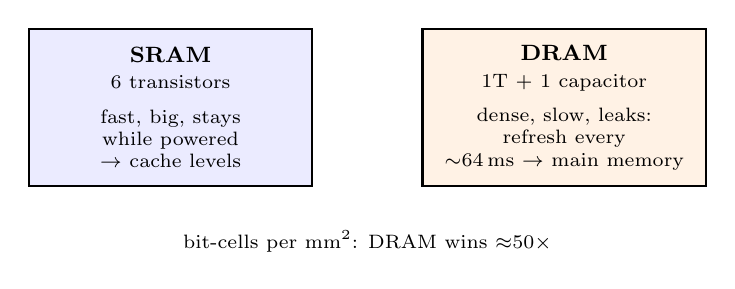
\begin{tikzpicture}[font=\footnotesize, x=1cm, y=1cm]
  \draw[thick, fill=blue!8] (0,1.6) rectangle (3.6,3.6);
  \node[align=center] at (1.8,3.1) {\textbf{SRAM}\\ \scriptsize 6 transistors};
  \node[align=center, font=\scriptsize] at (1.8,2.2)
    {fast, big, stays\\ while powered\\ $\to$ cache levels};
  \draw[thick, fill=orange!10] (5.0,1.6) rectangle (8.6,3.6);
  \node[align=center] at (6.8,3.1) {\textbf{DRAM}\\ \scriptsize 1T + 1 capacitor};
  \node[align=center, font=\scriptsize] at (6.8,2.2)
    {dense, slow, leaks:\\ refresh every\\ $\sim$64\,ms $\to$ main memory};
  \node[font=\scriptsize] at (4.3,0.9)
    {bit-cells per mm$^2$: DRAM wins $\approx$50$\times$};
\end{tikzpicture}
\caption{Why the hierarchy exists: the fast bit-cell (SRAM, 6T) is
physically too large to hold gigabytes, and the dense one (DRAM, 1T1C)
is too slow to feed a pipeline. Nobody picked this trade-off ---
physics did.}
\label{fig:sramdram09}
\end{figure}
